%---------------------------------------------------------------------------------------------------
% Introduction to the chapter
%---------------------------------------------------------------------------------------------------
\chapter{$f(Q)$ Cosmology with a $\Lambda$CDM Background}
\label{chap:STG-LCDM-bg}

In this chapter, we will study the most general $f(Q)$ modified gravity cosmological model which features a \gls{LCDM} background where the differences arise in the propagation of perturbations,
namely by introducing an effective gravitational constant. This model introduces only one additional free parameter, $\alpha$, which when set to zero makes this model fall back to \gls{LCDM}. Our main goal here is to assess the constraining power that both current and future \gls{GW} observatories will have in setting the boundaries on the parameter $\alpha$, by resorting to \gls{SS} mock catalogs.

This model has been the subject of study in previous original work carried out by the author in \cite{Ferreira2022}. This model has also been addressed in \cite{Barros2020}, where it has been shown to alleviate the $\sigma_8$ tension present in \gls{LCDM} and in \cite{Frusciante2021}, where an analysis using scalar angular power spectra, matter power and \glspl{GW} propagation was developed. Similar models were also briefly studied in \cite{Jimenez2017}, a more general model of the form $f(Q) = Q + \alpha Q^n$ was studied in \cite{Khyllep2021} and models of similar form were constrained using observational data in \cite{Ayuso2020, Atayde2021}.


%---------------------------------------------------------------------------------------------------
% The Model
%---------------------------------------------------------------------------------------------------
\section{The Model}
\label{sec:STG-LCDM-bg-model}

In order to ensure that our cosmological model of $f(Q)$ has a \gls{LCDM} background, we take the modified first Friedmann equation, presented in \cref{eq:STG-friedmann-1}, and set the right hand side to be equal to $H^2$. By making use of the relationship between the non-metricity scalar and the Hubble function, $Q = 6H^2$, we can then write

\begin{equation}
    Q f_Q - \frac{1}{2}f - \frac{Q}{2} = 0 \,,
\end{equation}
with, as shown in \cite{Jimenez2019}, the most general solution given by

\begin{equation}
    \label{eq:STG-LCDM-bg-model}
    f = Q + \alpha \sqrt{Q} \,,
\end{equation}
where $\alpha$ is an integration constant.

We will consider a universe which is composed of ordinary and dark matter, radiation and a cosmological constant. However, since the aim of this chapter is solely to forecast this model using \glspl{SS}, we can safely neglect radiation, as these objects are not expected to be detected at very high redshifts. Since the background is the same as \gls{LCDM}, we can make use of conservation laws and the Hubble function now reads

\begin{equation}
    H = H_0 \sqrt{\Omega_m (1+z)^3 + 1 - \Omega_m} \,.
\end{equation}

By inserting the specific form for this model, presented in \cref{eq:STG-LCDM-bg-model}, in the equation for the luminosity distance of \glspl{GW} in $f(Q)$, given in \cref{eq:STG-generic-dLGW}, the measured luminosity distance of a \gls{GW} is

\begin{equation}
    \label{eq:STG-LCDM-bg-dlgw}
    d_{\text{GW}}(z) = \sqrt{\frac{2\sqrt{6} + \alpha}{2\sqrt{6} + \alpha/E(z)}} \, d_L(z) \,,
\end{equation}
where $\alpha$ has been re-defined to be in units of $1/H_0$ and $E(z) \equiv H(z)/H_0$.

Looking at the previous equation, one can see that there is a singularity at $\alpha = -2\sqrt{6} E(z)$. To ensure that the value for the luminosity distance for \glspl{GW} is strictly physical (i.e. a real positive number for all redshifts), we must require that the value of $\alpha$ must have a lower bound at $\alpha = -2 \sqrt{6}$.


%---------------------------------------------------------------------------------------------------
% Forecasts using Standard Sirens
%---------------------------------------------------------------------------------------------------
\section{Forecasts using Standard Sirens}
\label{sec:STG-LCDM-bg-forecasts}

By looking at the expression for the luminosity distance of gravitational waves, as can be seen in \cref{eq:STG-LCDM-bg-dlgw}, we can see that this model features a degeneracy between two of its parameters, $\alpha$ and $\Omega_m$. In order to avoid problems with our sampler, we make use of the Pantheon sample with the marginalized \gls{SNIa} likelihood, developed in \cref{sec:SNIa}, to fix the value of $\Omega_m$. As such, besides the \glspl{SS} events, the Pantheon sample is present at all times.

\begin{figure}[h!]
    \centering
    \begin{subfigure}[t]{0.49\textwidth}
        \centering
        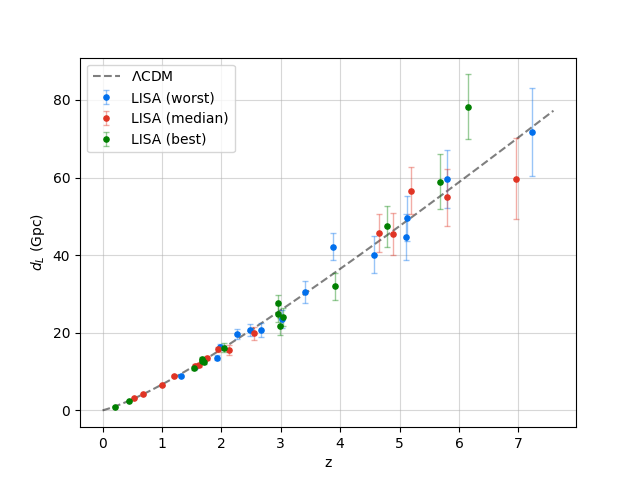
\includegraphics[width=\textwidth]{figures/LISA-9,10,12.png}
    \end{subfigure}
    \hfill
    \begin{subfigure}[t]{0.49\textwidth}
        \centering
        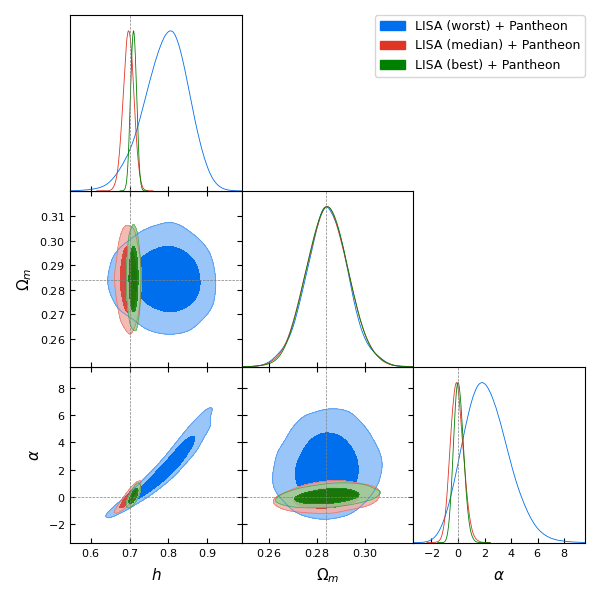
\includegraphics[width=\textwidth]{figures/fQ-LCDM-bg_LISA-9,10,12_pantheon-binned.png}
    \end{subfigure}
    \caption[The best, median and worst LISA catalogs represented in the luminosity distance versus redshift plane (left) and the corresponding constrains with the Pantheon sample set on the $f(Q)$ model with $\Lambda$CDM background (right). The fiducial $\Lambda$CDM cosmological model is plotted as a dashed gray line.]
    {The best, median and worst \gls{LISA} catalogs represented in the luminosity distance versus redshift plane (left) and the corresponding constrains with the Pantheon sample set on the model given by \cref{eq:STG-LCDM-bg-model} (right). The fiducial \gls{LCDM} cosmological model is plotted as a dashed gray line.}
    \label{fig:fQ-LCDM-bg_LISA}
\end{figure}

Starting the forecast with \gls{LISA}, we present in the left panel of \cref{fig:fQ-LCDM-bg_LISA} the best, median and worst \gls{LISA} catalogs, which are rated as previously described in \cref{chap:datasets}, on the luminosity distance versus redshift plane. On the right panel of the same figure, we show the corner plot illustrating the constrains on the parameters obtained by a joint analysis of the same catalogs, together with the Pantheon \gls{SNIa} data.

By looking at the constraints in the right plot of \cref{fig:fQ-LCDM-bg_LISA}, we can see that the worst catalog features significantly worst results when compared to both the median and best catalogs, which in turn are very similar when compared to each other. If we then look at the redshift distribution for the events presented in the left plot of \cref{fig:fQ-LCDM-bg_LISA}, we can see a pattern: the best catalog is the one which features events with the lowest redshifts, followed by the median catalog, and finally the worst catalog. From this fact, we infer that \gls{LISA} increases the quality of its constraints when the corresponding catalog features plenty of low redshift events.

Considering that, out of the 15 generated catalogs, only 2 provided error bars similar to the ones obtained in the worst catalog, we expect that the odds of obtaining a bad \gls{LISA} catalog to be low.

Focusing our attention on the \gls{ET}, we noticed that all of the 5 generated catalogs provide similar constraints. This is expected, as the number of events which we are considering for this observatory, $1000$ to be precise, is large enough to match the underlying statistical distribution. As such, we decided only to consider one \gls{ET} catalog, which we take as being representative of a whole range of outcomes for this observatory.

\begin{figure}[h!]
    \centering
    \begin{subfigure}[t]{0.49\textwidth}
        \centering
        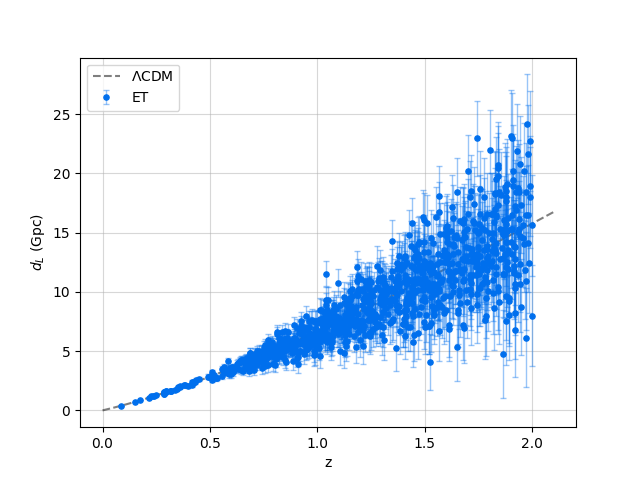
\includegraphics[width=\textwidth]{figures/ET-4.png}
    \end{subfigure}
    \hfill
    \begin{subfigure}[t]{0.49\textwidth}
        \centering
        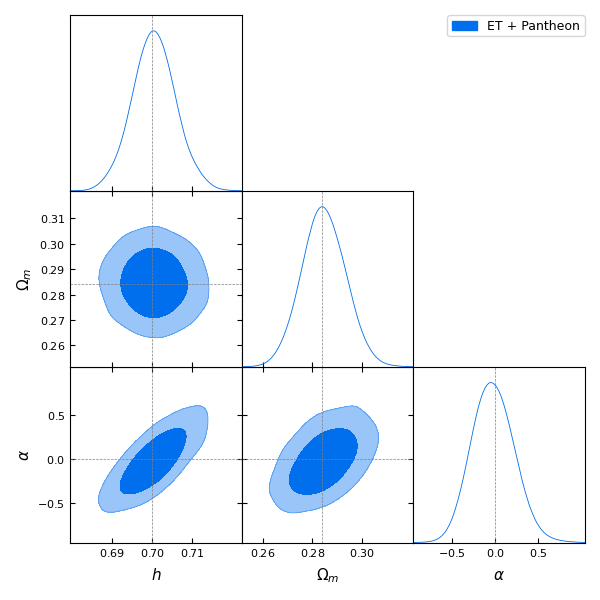
\includegraphics[width=\textwidth]{figures/fQ-LCDM-bg_ET-4_pantheon-binned.png}
    \end{subfigure}
    \caption[The considered ET catalog represented in the luminosity distance versus redshift plane (left) and the corresponding constrains with the Pantheon sample set on the $f(Q)$ model with $\Lambda$CDM background (right). The fiducial $\Lambda$CDM cosmological model is plotted as a dashed gray line.]
    {The considered \gls{ET} catalog represented in the luminosity distance versus redshift plane (left) and the corresponding constrains with the Pantheon sample set on the model given by \cref{eq:STG-LCDM-bg-model} (right). The fiducial \gls{LCDM} cosmological model is plotted as a dashed gray line.}
    \label{fig:fQ-LCDM-bg_ET}
\end{figure}

The single \gls{ET} catalog is presented in the left plot of \cref{fig:fQ-LCDM-bg_ET}, in the luminosity distance versus redshift plane, and the corresponding constraints for that catalog, when mixed with \gls{SNIa} obtained from the Pantheon sample, are presented in the right plot of \cref{fig:fQ-LCDM-bg_ET}.

If we are now to compare the constraints set by the \gls{ET} with the ones set by the best catalog \gls{LISA}, where both catalogs are presented in the left plot of \cref{fig:fQ-LCDM-bg_LISA_ET} and the corresponding constraints are presented in the right plot of \cref{fig:fQ-LCDM-bg_LISA_ET}.

\begin{figure}[h!]
    \centering
    \begin{subfigure}[b]{0.49\textwidth}
        \centering
        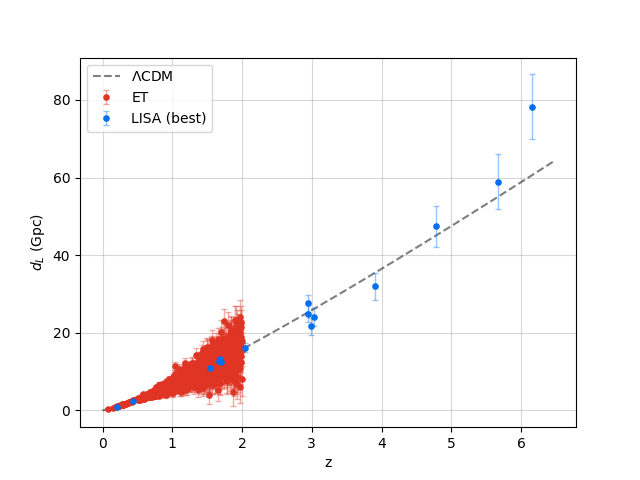
\includegraphics[width=\textwidth]{figures/ET-4,LISA-9.png}
    \end{subfigure}
    \hfill
    \begin{subfigure}[b]{0.49\textwidth}
        \centering
        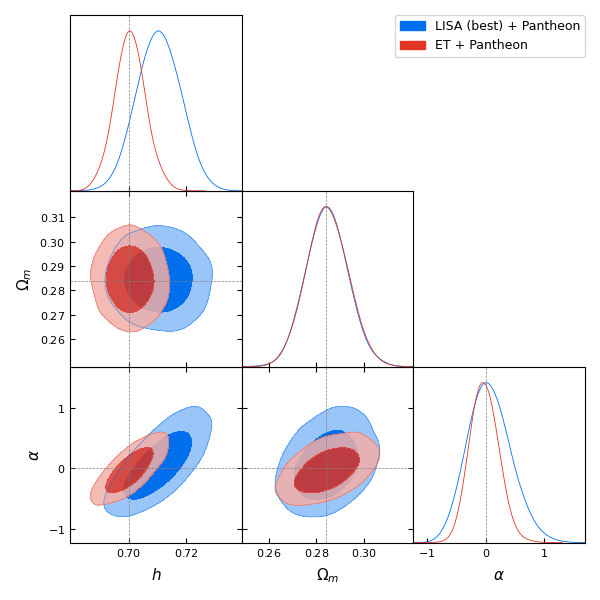
\includegraphics[width=\textwidth]{figures/fQ-LCDM-bg_ET-4,LISA-9_pantheon-binned.png}
    \end{subfigure}
    \caption[The considered ET catalog and the best LISA catalog represented in the luminosity distance versus redshift plane (left) and the corresponding constrains with the Pantheon sample set on the $f(Q)$ model with $\Lambda$CDM background (right). The fiducial $\Lambda$CDM cosmological model is plotted as a dashed gray line.]
    {The considered \gls{ET} catalog and the best \gls{LISA} catalog represented in the luminosity distance versus redshift plane (left) and the corresponding constrains with the Pantheon sample set on the model given by \cref{eq:STG-LCDM-bg-model} (right). The fiducial \gls{LCDM} cosmological model is plotted as a dashed gray line.}
    \label{fig:fQ-LCDM-bg_LISA_ET}
\end{figure}

By computing the area of the 1$\sigma$ region we can see that the best \gls{LISA} catalog has a region which is approximately 4 times bigger when compared to the one given by the \gls{ET}. The fact that the \gls{ET} will operate at significantly lower redshift when compared to \gls{LISA}, yet is able to provide better constraints, goes hand in hand with our previous statement regarding \gls{LISA} which is the fact that low redshift events are ideal to constrain this model. Granted, the \gls{ET} will provide a significantly larger number of events when compared to \gls{LISA}.

As for the \gls{LIGO}-Virgo collaboration, the forecasts indicate that these observatories are not able to constrain this model. As such, we have decided to categorize each \gls{LIGO}-Virgo catalog based on how well it complements the worst \gls{LISA} catalog. The worst \gls{LISA} catalog is chosen because both the best and median \gls{LISA} catalogs do not show significant improvements when added with any of the \gls{LIGO}-Virgo catalogs.

To understand why \gls{LIGO}-Virgo itself is not able to set proper constraints on our model, we refer to \cref{fig:LISA-9;LIGO-13;ET-4;low-redshifts}, where we can see a zoom of the events present in the low redshift regime, $z \in [0, 0.2]$, showcasing the best \gls{LIGO}-Virgo catalog, as well as the best \gls{LISA} catalog and the single \gls{ET} catalog. This plot shows that, although there is a much larger number of events, the \gls{LIGO}-Virgo error bars are significantly larger when compared to those of the \gls{ET} and \gls{LISA}.

\begin{figure}[h!]
    \centering
    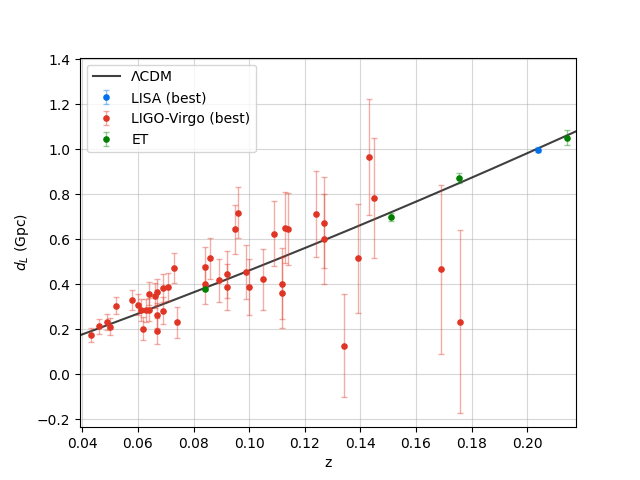
\includegraphics[width=0.65\columnwidth]{figures/LISA-9,LIGO-13,ET-4,low-redshifts.png}
    \caption[Luminosity distance, in Gpc, as a function of redshift for the best LISA catalog, the best LIGO-Virgo catalog and the ET catalog]
    {Luminosity distance, in Gpc, as a function of redshift, for the best \gls{LISA} catalog, the best \gls{LIGO}-Virgo catalog and the single \gls{ET} catalog. The $\Lambda$CDM luminosity distance is plotted as a solid gray line.}
    \label{fig:LISA-9;LIGO-13;ET-4;low-redshifts}
\end{figure}

The forecasts set by \gls{LIGO}-Virgo, when joined together with the worst \gls{LISA} catalog and the \gls{SNIa} from the Pantheon sample, are presented in \cref{fig:FQ_LISA-12_SNIa-binned_none;LIGO-1;2;13}. These results reveal that if the events observed by \gls{LISA} resembles a worst \gls{LISA} catalog, \gls{LIGO}-Virgo is expected to significantly increase the quality of the constraints, and approximate its constraining power to that of a median \gls{LISA} catalog.

\begin{figure}[h!]
    \centering
    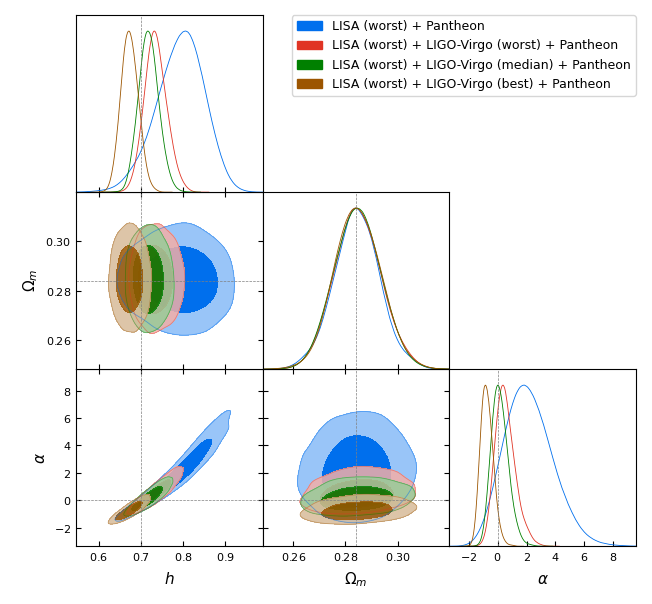
\includegraphics[width=0.65\columnwidth]{figures/fQ-LCDM-bg_LISA-12_LIGO-1,2,13_pantheon-binned.png}
    \caption[Constraints set by the worst, median and best LIGO catalogs, when joined together with the worst LISA catalog and data from the Pantheon dataset, for the most general model of $f(Q)$ with a $\Lambda$CDM backgroun. The worst \gls{LISA} catalog with Pantheon is also shown for comparison.]
    {Constraints set by the worst, median and best \gls{LIGO} catalogs, when mixed together with the worst \gls{LISA} catalog and data from the Pantheon dataset, for the model given by \cref{eq:STG-LCDM-bg-model}. The worst \gls{LISA} catalog with Pantheon is also shown for comparison. Dotted lines represent the fiducial \gls{LCDM} values.}
    \label{fig:FQ_LISA-12_SNIa-binned_none;LIGO-1;2;13}
\end{figure}

In an attempt to further increase the quality of our constraints with the available catalogs, we added each of the \gls{LISA} catalogs with the single \gls{ET} catalog, where only the best \gls{LISA} catalog showed non-negligible improvements. As for the data of \gls{LIGO}-Virgo when mixed with the \gls{ET}, no significant improvements were observed. These results were to be expected given by both the high quality of the constraints and the number of events measured by the \gls{ET}.

The results set by \gls{LISA} show that, even though the luminosity distance for this model deviates from that of \gls{LCDM} as the redshift increases, the error bars increase faster, in such a way that high redshift events are less useful to constrain this model. On the other hand, were we to observe an event at the very low redshifts with a larger error bar, as was clearly seen for the case of \gls{LIGO}-Virgo, then we would be unable to set proper constraints. We also saw that this is also true for \gls{LISA}, since in this regime the current model is practically indistinguishable from \gls{LCDM} and, to further complicate matters, the observations are more sensitive to the peculiar velocities, consequently increasing the error bars of our measurements.

We noted that the value for the 1$\sigma$ region for the parameter $h$, which we label as $\sigma_h$, is approximately linear with the 1$\sigma$ region for the parameter $\alpha$, labeled as $\sigma_\alpha$. We would also like to note that the value for $\Omega_m$, as well as its error $\sigma_{\Omega_m}$, are the same for all catalogs regardless of the observatory considered. This is due to the usage of \gls{SNIa} that fixes the value of $\Omega_m$. As such, without losing any information with respect to the quality of the constrains on the other parameters, we can categorize each catalog based on the value of $\sigma_\alpha$.

In \cref{tab:fQ-LCDM-bg-constrains} we show the value of $\sigma_\alpha$ for the more relevant cases, by decreasing order of constraining power, as well as the relative size of each region with respect to the best expected outcome.

\begin{table}[h!]
\centering
\begin{tabular}{|c|c|c|}
\hline
Catalog                          & $\sigma_\alpha$ & Relative Size \\ \hline
ET                               & 0.25            & 1             \\ \hline
LISA (best)                      & 0.37            & 1.5           \\ \hline
LISA (worst) + LIGO-Virgo (best) & 0.44            & 1.8           \\ \hline
LISA (median)                    & 0.49            & 2             \\ \hline
LISA (worst)                     & 1.70            & 6.8           \\ \hline
\end{tabular}
\caption{Summary of the size of the 1$\sigma$ region for the parameter $\alpha$, labeled as $\sigma_\alpha$, for the more relevant cases, ordered by decreasing constraining power. The relative size of $\sigma_\alpha$ for each case compare to the best expected outcome is also presented.}
\label{tab:fQ-LCDM-bg-constrains}
\end{table}

Quantitatively, \cref{tab:fQ-LCDM-bg-constrains} shows that we can expect that the \gls{ET} will be able to measure the value of $\alpha$ with a 1$\sigma$ region of $0.25$. Then, our most optimistic result for \gls{LISA} shows that it will be able to set the bounds on $\alpha$ on a region which is 0.5 larger than that of the \gls{ET}. If instead we are to observe a bad \gls{LISA} catalog, then we expect to have a 1$\sigma$ region which is almost 7 times worst when compared to the \gls{ET}. However, if we are to measure the equivalent of the best case for \gls{LIGO}-Virgo, the quality of those constrain will be able to improve enormously to reveal only 0.8 worst when compared to the \gls{ET}. This last case, although features a bad \gls{LISA} catalog, it is slightly better when compared to the median \gls{LISA} catalog, which will be 2 times worst compared to the \gls{ET}.


%---------------------------------------------------------------------------------------------------
% Summary
%---------------------------------------------------------------------------------------------------
\section{Summary}
\label{sec:STG-LCDM-bg-summary}

In this chapter, we have considered the most general model of $f(Q)$ gravity that mimics a \gls{LCDM} background, which introduces one additional free parameter. Due to this choice of background, departures from \gls{LCDM} only arise at the perturbative level.

We forecast this model using \gls{SS} mock catalogs generated for \gls{LISA}, \gls{ET} and \gls{LIGO}-Virgo. Additionally, due to a degeneracy between two of the model parameters, each mock catalog was constrained in conjunction with \gls{SNIa} from the Pantheon sample.

The \gls{LISA} catalog which provided the best constraints is the one which features more events at low redshifts, while the worst catalog is composed mostly of high redshift events, and the median is somewhere in between. This result indicates that, even though our model deviates more from \gls{LCDM} as the redshift increase, the error bars increase faster, making high redshift observations less useful to provide constraints. Based on all of the generated \gls{LISA} catalogs, a catalog which provides similar constraints to the worst \gls{LISA} catalog is not very likely to be observed.

For the \gls{ET} it was observed that all catalogs provide similar constraints and as such only had to consider one catalog to be representative of the whole set. This is expected since each catalog features 1000 \gls{SS} events, a number which is large enough to represent the underlying probability distribution function. On top of this consistency, the \gls{ET} performs slightly better than the best \gls{LISA} catalog.

As for \gls{LIGO}-Virgo, we observed that a dataset consisting of 50 \glspl{SS} events are not enough to provide meaningful constraints. Instead, we categorized each \gls{LIGO}-Virgo catalog based on how well it would complement the worst \gls{LISA} catalog. We showed that one can rely on future events obtained by \gls{LIGO}-Virgo to improve the quality of the constraints, meaning that, in the future, if we obtain a catalog similar to that of a worst \gls{LISA} catalog, we can use data from \gls{LIGO}-Virgo to approximate it to have the quality of a median \gls{LISA} catalog. By contrast, for both the best or the median \gls{LISA} catalogs, none of the \gls{LIGO}-Virgo catalogs made significant improvements on the results.

We can provide small improvements to the constraints set by the \gls{ET} using the best \gls{LISA} catalog. By contrast, the median and the worst \gls{LISA} catalog, as well as any of the \gls{LIGO}-Virgo catalogs, make no significant improvements when constrained together with the \gls{ET}.

We observed that the size of the 1$\sigma$ region for $\alpha$ has a quasi-linear relationship with the size of the 1$\sigma$ region for $h$. Due to the fact that the parameter $\Omega_m$ was fixed by the usage of \gls{SNIa}, we were able to rate the quality of the constrains of each catalog based only on the size of $\sigma_\alpha$, without losing information regarding the quality of the constrains of the other parameters.

In \cref{tab:fQ-LCDM-bg-constrains} we summarize the forecasts of the constrains set on the parameter $\alpha$ for the more relevant cases we have studied. Quantitatively, we show that the \gls{ET} will be able to set a 1$\sigma$ region for the parameter $\alpha$ of size 0.25, whereas the best possible scenario for \gls{LISA} shows a region which is about 0.5 larger. The median \gls{LISA} catalog showed a 1$\sigma$ region which is 2 times larger, again compared with the constrains set by the \gls{ET}, while the worst possible case expected for \gls{LISA} revealed a region which is almost 7 times larger. Fortunately, the data from \gls{LIGO}-Virgo is expected to improve the quality of the constrains, which in a best case scenario is expected to improve the size of the 1$\sigma$ region from 7 times larger to only 0.8 times worst when compared to the \gls{ET}, beating the result set by a median \gls{LISA} catalog.
